\documentclass{article}


% if you need to pass options to natbib, use, e.g.:
%     \PassOptionsToPackage{numbers, compress}{natbib}
% before loading neurips_2022


% ready for submission
\usepackage[preprint,nonatbib]{neurips_2022}


% to compile a preprint version, e.g., for submission to arXiv, add add the
% [preprint] option:
%     \usepackage[preprint]{neurips_2022}


% to compile a camera-ready version, add the [final] option, e.g.:
%     \usepackage[final]{neurips_2022}


% to avoid loading the natbib package, add option nonatbib:
%    \usepackage[nonatbib]{neurips_2022}


\usepackage[utf8]{inputenc} % allow utf-8 input
\usepackage[T1]{fontenc}    % use 8-bit T1 fonts
\usepackage{hyperref}       % hyperlinks
\usepackage{url}            % simple URL typesetting
\usepackage{booktabs}       % professional-quality tables
\usepackage{amsfonts}       % blackboard math symbols
\usepackage{amsmath}
\usepackage{amsthm}
\usepackage{nicefrac}       % compact symbols for 1/2, etc.
\usepackage{microtype}      % microtypography
\usepackage{xcolor}         % colors
\usepackage[backend=biber, sorting=none]{biblatex}
\usepackage{graphicx}
\usepackage{subcaption}

\newtheorem{assumption}{Assumption}
\newtheorem{definition}{Definition}
\newtheorem{theorem}{Theorem}

\addbibresource{reference.bib}


\title{Direct Runge-Kutta Discretization Achieves Acceleration}


% The \author macro works with any number of authors. There are two commands
% used to separate the names and addresses of multiple authors: \And and \AND.
%
% Using \And between authors leaves it to LaTeX to determine where to break the
% lines. Using \AND forces a line break at that point. So, if LaTeX puts 3 of 4
% authors names on the first line, and the last on the second line, try using
% \AND instead of \And before the third author name.


\author{%
  Xiaoxuan Yu \\
  College of Chemistry and Molecular Engineering\\
  Peking University\\
  Beijing, China \\
  \texttt{xiaoxuan\_yu@pku.edu.cn} \\
  % examples of more authors
  \And
  Yihang Xia \\
  School of Mathematical Sciences \\
  Peking University \\
  Beijing, China\\
  \texttt{xyh-mathematics@pku.edu.cn} \\
  \And
  Fabrice Sashinkumar \\
  Guanghua School Of Management - Exchange Student  \\
  Peking University \\
  Beijing, China \\
  \texttt{fabrice@stu.pku.edu.cn} \\
}


\begin{document}


\maketitle


%\section{Overview}
%\label{overview}

\section{Problem setup and backgrounds}

The article \cite{NEURIPS2018_44968aec} studies gradient-based optimization methods obtained by directly
discretizinga second-order ordinary differential equation (ODE) related to the
continuous limit of Nesterov's accelerated gradient method. It introduces some
conditions under which the sequence of iterates generated by discretizing the
proposed second-order ODE converges to the optimal solution at a certain rate.\\\\
Firstly let's focus the essential target problem:
\begin{align}\label{min}
  \mathop{\mathrm{min}}\limits_{x \in \mathbb{R}^{d}} f(x),
\end{align}
where $f$ is convex and sufficiently smooth. For solving \eqref{min}, there are several
methods.
\begin{itemize}
  \item Classical method: gradient decent, which displays a sub-optimal convergence rate of $\mathcal{O}(N^{-1})$.
  \item Nesterov's seminal accelerated gradient method, matches the oracle lower bound of $\mathcal{O}(N^{-2})$.
\end{itemize}
Several articles have pursued approaches to NAG (and accelerated methods in general)
via a continuous-time perspective. However, they fail to provide a general
discretization procedure that generates provably convergent accelerated methods.
This article takes Runge-Kutta integrater as tool and introduces a second-order ODE
that generates an accelerated first-order method for smooth functions if using
Runge-Kutta method.\\\\

\section{Main results}
To build up a iterative method, letting $x_{0}$ be the initial point, firstly we
consider the sublevel set
\begin{align}\label{sublevel_set}
  \mathcal{S} := \{ x \in \mathbb{R}^{d} | f(x) \leq \mathrm{exp}(1) (f(x_{0})
  - f(x^{*}) + \|x_{0} - x^{*}\|^{2}) + 1 \},
\end{align}
where $x^{*}$ is the minimum of \eqref{min}. The introduction of set $\mathcal{S}$
actually gives a restriction of the sequence of iterates obtained from
discretizing a suitable ODE (would be proved later). Denote subset
\begin{align}
  \mathcal{A} := \{ x \in \mathbb{R}^{d} | \exists x' \in \mathcal{S}, \|x-x'\| \leq 1 \},
\end{align}
Then all assumptions we may require can be considered just in $\mathcal{A}$.

\begin{assumption}\label{assumption1}
  There exists an integer $p \geq 2$ and a positive constant L such that for any point $x \in \mathcal{A}$, and for all indices $i \in \{1,\ldots,p-1\}$, we have the lower-bound
  \begin{align}\label{assum_1}
    f(x) - f(x^{*}) \geq \frac{1}{L} \| \nabla^{(i)}f(x) \|^{\frac{p}{p-i}},
  \end{align}
  where $x^{*}$ minimizes f and $\| \nabla^{(i)}f(x) \|$ denotes the operator norm of the tensor $\nabla^{(i)}f(x)$.
\end{assumption}

\begin{assumption}\label{assumption2}
  There exists an integer $s \geq p$ and a constant $M \geq 0$, such that $f(x)$ is order $(s+2)$ differentiable. Furthermore, for any $x \in \mathcal{A}$, the following operator norm bounds hold:
  \begin{align}\label{assum_2}
    \| \nabla^{(i)}f(x) \| \leq M,\ \text{for}\ i = p,p+1,\ldots,s,s+1,s+2.
  \end{align}
\end{assumption}

When the sublevel sets of $f$ are compact and hence the set $\mathcal{A}$ is also compact; as a result, the bound \eqref{assum_2} on high order derivatives is implied by continuity.

\subsection{Runge-Kutta\ integrators}

The explicit Runge-Kutta integrators used in the article appears in the form below.

\begin{definition}
  Given a dynamical system $\dot{y} = F(y)$, let the current point be $y_{0}$ and the step size be $h$. An explicit $S$ stage Runge-Kutta method generates the next step via the following update:
  \begin{align}\label{def_1}
    g_{i} = y_{0} + h \sum\limits_{j=1}^{i-1} a_{ij}F(g_{j}),\ \ \ \Phi_{h}(y_{0}) = y_{0}
    + h \sum\limits_{i=1}^{S} b_{i}F(g_{i}),
  \end{align}
  where $a_{ij}$ and $b_{i}$ are suitable coefficients defined by the integrator; $\Phi_{h}(y_{0})$ is the estimation of the state after time step $h$, while $g_i$ (for $i = 1,\ldots,S$) are a few neighboring points where the gradient information $F(g_i)$ is evaluated.
\end{definition}

In general, Runge-Kutta methods offer a powerful class of numerical integrators, and with the knowledge
of its concergence behaviour when discretizing for solutions, the article gets to use it
to discretize ODE with controlment of its convergence rates.

\subsection{Formal work and inspiration}

Then focus on the NAG method that is defined according to the updates
\begin{align}\label{nag}
  x_{k} = y_{k-1} - h \nabla f(y_{k-1}),\ \ \ y_{k} = x_{k} + \frac{k-1}{k+2} (x_{k} - x_{k-1}).
\end{align}
\textcite{JMLR:v17:15-084} showed that the iteration \eqref{nag} in the limit is equivalent to the
following ODE
\begin{align}\label{nag_ode_1}
  \ddot{x}(t) + \frac{3}{t} \dot{x}(t) + \nabla f(x(t)) = 0,\ \ \ \mathrm{where\ }
  \dot{x} = \frac{dx}{dt}
\end{align}
when one drives the step size $h$ to zero. It can be further shown that in the
continuous domain the function value $f(x(t))$ decreases at the rate of $\mathcal{O}(1/t2)$
along the trajectories of the ODE. This convergence rate can be accelerated to an
arbitrary rate in continuous time via time dilation as in [Wibisono et al., 2016].
In particular, the solution to
\begin{align}\label{nag_ode_2}
  \ddot{x}(t) + \frac{p+1}{t} \dot{x}(t) + p^{2}t^{p-2} \nabla f(x(t)) = 0
\end{align}
has a convergence rate $\mathcal{O}(1/t^{p})$. When $p > 2$, Wibisono et al. [2016] proposed rate matching
algorithms via utilizing higher order derivatives. However, this article focuses purely on
first-order methods and study the stability of discretizing the ODE directly when
$p \geq 2$.
\\\\According to some related work, deriving the ODE from the algorithm is now a solved
problem. Nevertheless, to derive the update of NAG or any other
accelerated method by directly discretizing an ODE is not. Some work points out that
explicit Euler discretization of the ODE in \eqref{nag_ode_1} may not lead to a stable
algorithm. \textcite{https://doi.org/10.48550/arxiv.1802.03653} observed empirically that Verlet
integration is stable and suggested that the stability relates to the symplectic
property of the Verlet integration, but for dissipative systems such as \eqref{nag_ode_2},
this doesn't hold. This article offers a different approach: it augments the state with
time in \eqref{nag_ode_2}, and focuses the following ODE
\begin{align}\label{nag_ode_final}
  \ddot{x}(t) + \frac{2p+1}{t} \dot{x}(t) + p^{2}t^{p-2} \nabla f(x(t)) = 0.
\end{align}
This actually turns the non-autonomous dynamical system into an autonomous one.

\subsection{Main\ conclusion}

The ODE in \eqref{nag_ode_final} can also be written as the dynamical system
\begin{align}\label{equation}
  \dot{y} = F(y) = \begin{bmatrix}
                     -\frac{2p+1}{t} v - p^{2}t^{p-2} \nabla f(x) \\
                     v                                            \\
                     1
                   \end{bmatrix},\ \ \ \mathrm{where\ }y = [v;x;t].
\end{align}
\textbf{Algorithm\ 1:\ }Input$(f,x_{0},p,L,M,s,N)$ \hfill $\triangleright$ Constants
$p,L,M$ are the same as in Assumptions\\
1. Set the initial state $y_{0} = [\overrightarrow{0};x_{0};1] \in \mathbb{R}^{2d+1}$\\
2. Set step size $h = C/N^{(1/s+1)}$ \hfill $\triangleright$ C is determined by
$p,L,M,s,x_{0}$\\
3. $x_{N} \leftarrow $ Oreder-s-Runge-Kutta-Integrater($F,y_{0},N,h$) \hfill $\triangleright$
F is defined in equation \eqref{equation}\\
4. \textbf{return} $x_{N}$\\\\
Since the article has augmented the state with time to obtain an autonomous system,
it can be readily solved numerically with a Runge-Kutta integrator as in
\textbf{Algorithm 1}.

\begin{theorem}\label{theorem}
  Consider the second-order ODE in \eqref{nag_ode_final}. Suppose that the function $f$ is convex and Assumptions 1 and 2 are satisfied. Further, let s be the order of the Runge-Kutta integrator used in \textbf{Algorithm 1}, $N$ be the total number of iterations, and $x_0$ be the initial point. Also, let $\mathcal{E}_{0} := f(x_{0}) - f(x^{*}) + \|x_{0} - x^{*}\|^{2} + 1$. Then, there exists a constant $C_1$ such that if we set the step size as $h = C_{1}N^{-1/(s+1)} (L+M+1)^{-1}\mathcal{E}_{0}^{-1}$, the iterate $x_N$ generated after running \textbf{Algorithm 1} for N iterations satisfies the inequality
  \begin{align}\label{thereom_1}
    f(x_{N}) - f(x^{*}) \leq C_{2}\mathcal{E}_{0} \left[
      \frac{(L+M+1)\mathcal{E}_{0}}{N^{\frac{s}{s+1}}} \right]^{p} = \mathcal{O}
    (N^{-p\frac{s}{s+1}}),
  \end{align}
  where the constants C1 and C2 only depend on $s, p$, and the Runge-Kutta integrator. Since each iteration consumes S gradient, $f(x_N) - f(x^{*})$ will converge as $\mathcal{O}(S^{\frac{ps}{s+1}}N^{-\frac{ps}{s+1}})$ with respect to the number of gradient evaluations. Note that for commonly used Runge-Kutta integrators, $S \leq 8$.
\end{theorem}
% \subsubsection*{Application to logistic loss}
\section{Proof}
In this section we're going to explore the proof of Theorem \ref{theorem}, the details of the proof is included in Appendix \ref{proof}.
\subsection{Summary}
\begin{itemize}
    \item The proof begins by defining a Lyapunov function $\mathcal{E}$ that quantifies progress and shows that it is monotonically non-increasing along the continuous trajectory of the ODE. This means that the value of the Lyapunov function is always decreasing or remaining the same along the trajectory, which implies that the suboptimality of the solution $f(x) - f(x^*)$ and the norm of the gradient $v$ are bounded above by some constants.

    \item The proof then focuses on bounding the distance between the points in the discretized and continuous trajectories. This is done by showing that the difference between the two points is bounded by the step size of the numerical integrator. Specifically, it is shown that there exists a constant $C_1$ such that the distance between the points is bounded by $C_1 h^{s+1}$, where $h$ is the step size and $s$ is the order of the Runge-Kutta integrator.

    \item Using the bound on the distance between the points in the discretized and continuous trajectories, the proof then shows that the Lyapunov function is also monotonically non-increasing along the discretized trajectory. This means that the value of the Lyapunov function is always decreasing or remaining the same along the discretized trajectory, which implies that the suboptimality of the solution is also decreasing or remaining the same.

    \item Finally, the proof uses the continuity of the Lyapunov function and the bound on the distance between the points in the discretized and continuous trajectories to show that the suboptimality of the discretized sequence of points also converges to zero quickly. Specifically, it is shown that there exists a constant $C_2$ such that the suboptimality of the discretized sequence of points is bounded by $C_2 \mathcal{E}_0 [(L+M+1)\mathcal{E}_0/N^{s/(s+1)}]^p$, where $\mathcal{E}_0$ is the initial value of the Lyapunov function, $N$ is the total number of iterations, and $p$ is a positive constant that depends on the order of differentiability of the objective function. This result implies that the suboptimality of the discretized sequence of points converges to zero at a rate that is close to $O(N^{-p})$ with respect to the number of gradient evaluations.
\end{itemize}

\subsection{Comments}
\begin{itemize}
    \item The proof relies on the assumption that the objective function $f$ is convex and satisfies certain conditions on its derivatives, which are stated as Assumptions \ref{assumption1} and \ref{assumption2} in the theorem. These assumptions are necessary for the Lyapunov function to be monotonically non-increasing along the continuous trajectory of the ODE and for the suboptimality of the solution to converge to zero.

    \item The bound on the distance between the points in the discretized and continuous trajectories depends on the order of the Runge-Kutta integrator used. Higher-order integrators can provide a tighter bound, which leads to a faster convergence rate for the suboptimality of the discretized sequence of points.

    \item The theorem states that the Direct Runge-Kutta Discretization method can achieve a convergence rate that is close to $O(N^{-p})$ with respect to the number of gradient evaluations, where $N$ is the total number of iterations and $p$ is a positive constant that depends on the order of differentiability of the objective function. This convergence rate is faster than the $O(N^{-1})$ rate which is typically achieved by first-order methods such as gradient descent.

    \item One possible remark is that the constants $C_1$ and $C_2$ in the proof depend on the order of the Runge-Kutta integrator and the positive constant $p$ that depends on the order of differentiability of the objective function. These constants can affect the convergence rate of the algorithm and the step size $h$ that needs to be chosen. In particular, choosing a higher order integrator or a higher order of differentiability may lead to better convergence rates, but also requires a smaller step size to achieve these rates. On the other hand, choosing a smaller step size may increase the computational cost of the algorithm. It is important to carefully balance these trade-offs in practice to achieve good performance.

    \item Another remark is that the proof assumes the existence of a solution $x^*$ that minimizes the objective function $f(x)$. This assumption is necessary for the Lyapunov function $\mathcal{E}$ to be well-defined and for the convergence result to hold. In practice, it may be challenging to verify the existence of such a solution, especially when the objective function is nonconvex. In these cases, it is important to carefully choose the initial point $x_0$ and the step size $h$ to ensure that the algorithm converges to a good approximate solution.

    \item Finally, it is worth noting that the proof of Theorem 1 relies on several technical assumptions, such as convexity of the objective function, Lipschitz continuity of the gradient, and boundedness of high order derivatives. These assumptions are typically required to establish convergence results for optimization algorithms, but may not always hold in practice. It is important to carefully verify these assumptions before applying the algorithm and to choose appropriate algorithms or methods if these assumptions are not satisfied.

\end{itemize}
\subsection{Further improvements}
\begin{itemize}
    \item One additional point that may be helpful in understanding the proof is that the Lyapunov function is used to quantify the progress of the algorithm in terms of the suboptimality of the solution and the norm of the gradient. The monotonicity of the Lyapunov function along the continuous and discretized trajectories implies that these quantities are non-increasing, which in turn implies that the algorithm is making progress towards the optimal solution.

    \item Another point to consider is that the proof relies on the existence of a constant $C_1$ such that the distance between the points in the discretized and continuous trajectories is bounded by $C_1 h^{s+1}$. This constant is not explicitly calculated in the proof, but it is stated that replacing $C_1$ with any smaller positive constant leads to the same polynomial rate of convergence. This means that the specific value of $C_1$ is not important for achieving the desired convergence rate, as long as it is small enough.
\end{itemize}

\section{Numerical Experiments}
In this section, we implement the algorithms in the original article with \texttt{Julia} and its package \texttt{DifferentialEquations.jl} \cite{rackauckas2017differentialequations}. By comparing ODE direct discretizating (DD) methods described in the article against gradient descent (GD) and Nesterov's accelerated gradient (NAG) methods, we can verify the main results in the theoretical part. The code of these experiments can be found here: \url{https://github.com/xiaoxuan-yu/Direct-Runge-Kutta-Discretization-Achieves-Acceleration-PKU}.

Inspired by the numerical results by \textcite{NEURIPS2019_7a2b33c6}, we generate normal distributed separable dataset and fit a linear model \(Ax=b\). Then, we minimize three different kinds of loss functions:
\begin{equation}
    \begin{aligned}
        f_1(x) & = \left\| Ax-b \right\|_{2}^2                \\
        f_2(x) & = \sum_{i}\log(1+e^{-w_i^{\mathrm{T}}x y_i}) \\
        f_3(x) & = \frac{1}{4}\left\| Ax-b \right\|_{4}^4
    \end{aligned}
\end{equation}
where $f_1(\cdot ),f_2(\cdot ),f_3(\cdot )$ are $L_2$ loss, logistic loss and $L_4$ loss, respectively. For each test case and optimization algorithm, we empirically select the learning rate as the largest step length among $\{ 10^{-k}|k\in \mathbb{Z} \}$ that the method remains stable during the optimization process. Main results are shown in Figure \ref{Numerical} where all figures are on log-log scale.
\begin{figure}[htbp]
    \begin{subfigure}{0.45\textwidth}
        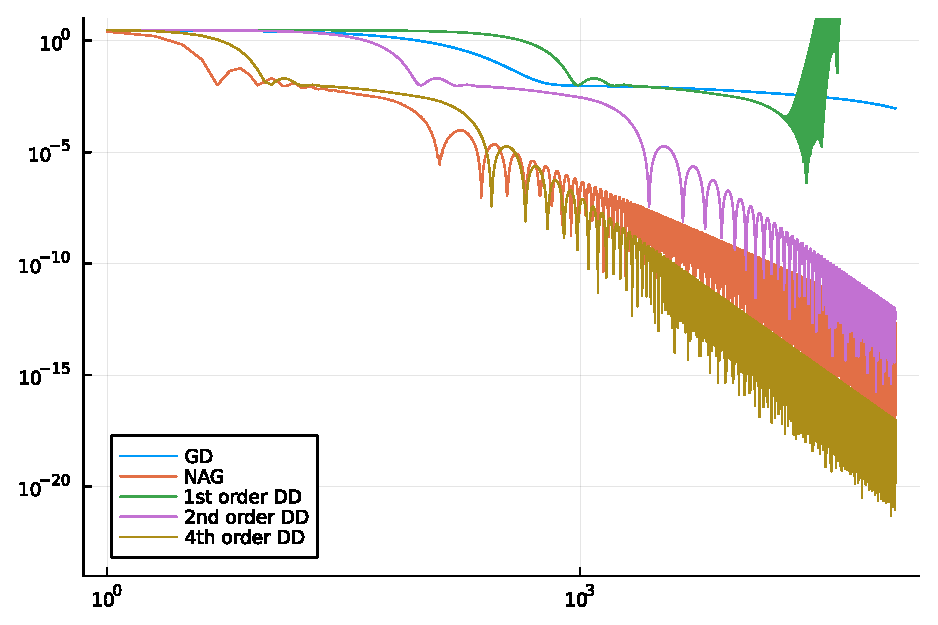
\includegraphics[width=\textwidth]{"assets/quadratic-1.pdf"}
        \caption{}
        \label{fig:l2-1}
    \end{subfigure}
    \hfill
    \begin{subfigure}{0.45\textwidth}
        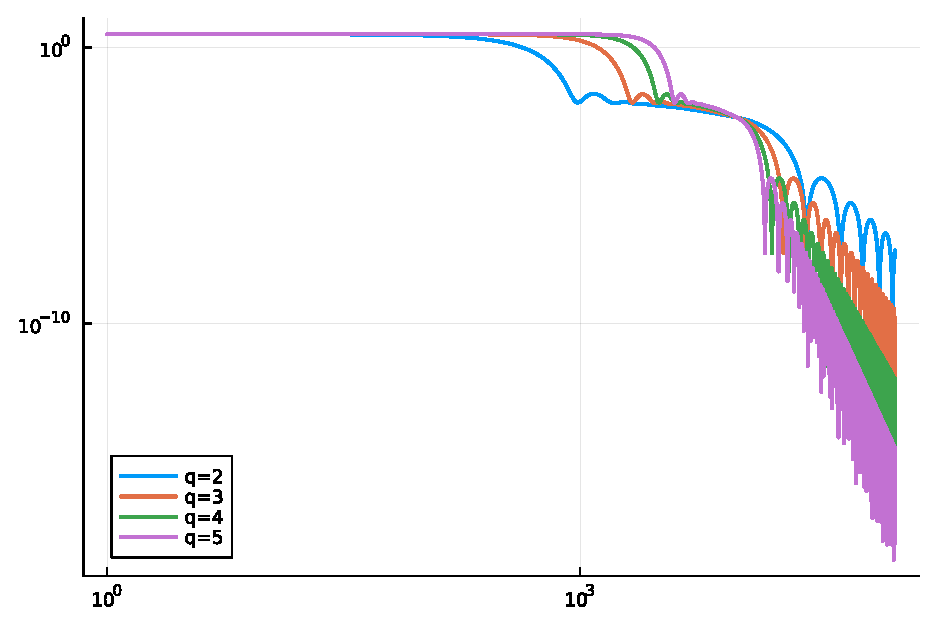
\includegraphics[width=\textwidth]{"assets/quadratic-2.pdf"}
        \caption{}
        \label{fig:l2-2}
    \end{subfigure}
    \hfill
    \begin{subfigure}{0.45\textwidth}
        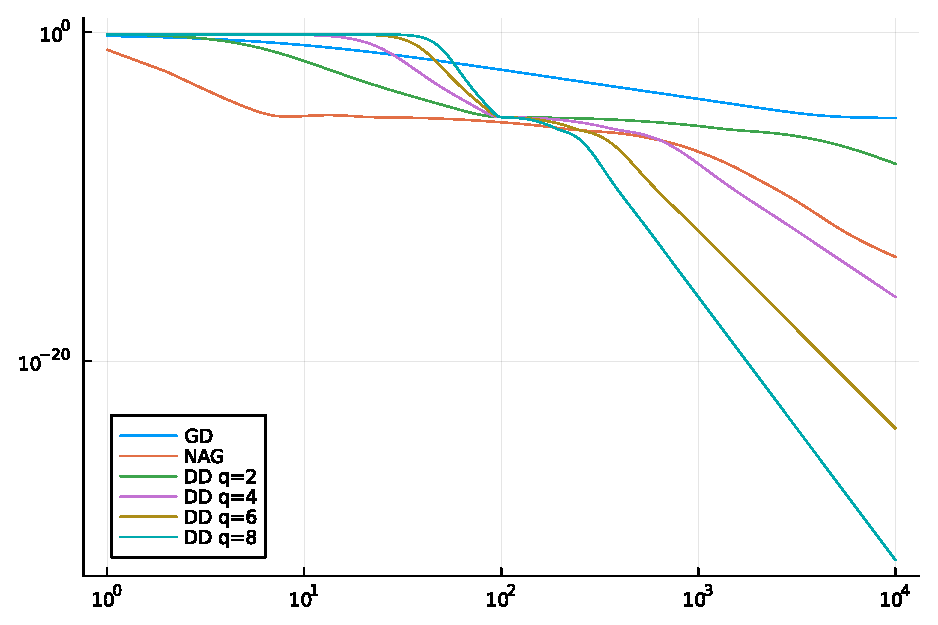
\includegraphics[width=\textwidth]{"assets/l4loss.pdf"}
        \caption{}
        \label{l4}
    \end{subfigure}
    \hfill
    \begin{subfigure}{0.45\textwidth}
        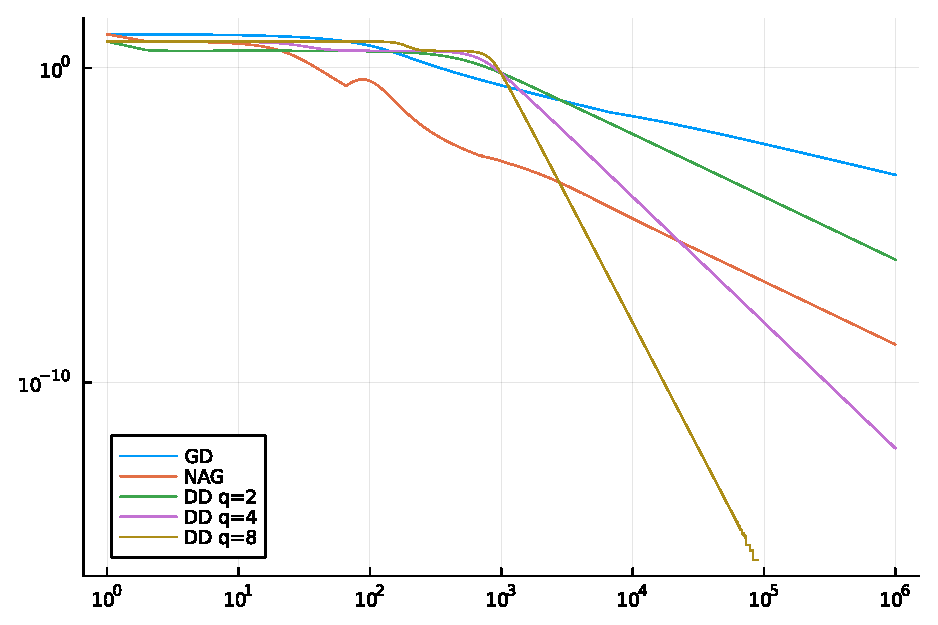
\includegraphics[width=\textwidth]{"assets/logistic.pdf"}
        \caption{}
        \label{fig:logistic}
    \end{subfigure}
    \caption{Experimental results comparing DD with GD and NAG. (a) Convergence path of GD, NAG and DD with different Runge-Kutta integrators of degree $s=1, 2, 4$ on $L_2$ loss. (b) The optimization of $L_2$ loss by DD with different choices of $q$ values with 4-th order Runge-Kutta integrator RK4. (c) Minimization of $L_4$ loss by GD, NAG and DD with different $q$ vaues with a 2-nd order Runge-Kutta integrator. (d) Minimization of logistic loss by GD, NAG and DD with different $q$ vaues with a 4-th order Runge-Kutta integrator.}
    \label{Numerical}
\end{figure}

First, we explore the optimization path of a quadratic function, the $L_2$ loss, with respecct to iteration. In particular, we labeled half of the generated data by 0 and the rest by 1. In Figure \ref{fig:l2-1}, the ODE is discretized for $p=2$ with different Runge-Kutta integrators with $s \in \{ 1,2,4 \}$ and compared against GD and NAG algorithm. We can find that except the integrator with $s=1$ can not converge due to the unstability of the differential format itself, the DD methods shows superiority over GD. By using higher order iterator, the local acceleration is achieved and 4th order DD even converges faster than NAG (although for each iteration, it is obviously more costly than NAG). In Figure \ref{fig:l2-2}, we explore the effect of $q$ is the ODE. Since in the article $p$ keeps the same as the one in Assumption \ref{assumption1}, thus we denotes $q$ the true parameter used in the ODE as below
$$
    \ddot x(t) + \frac{2q+1}{t}\dot x(t)+q^2 t^{q-2}\nabla  f(x(t)) = 0.
$$
We optimize the same $L_2$ loss with different values of $q$. By selecting smaller learning rates and increasing the numerical precision by using longer floats, the phenomenon that DD method diverges when $q>2$ is not observed. Instead, we found that for $q \in \{ 2,3,4,5 \}$, larger $q$ will give out faster convergence.

Then the minimization of $L_4$ loss (Figure \ref{l4}) and logistic loss (Figure \ref{fig:logistic}) is studied. We use 2-nd order Runge-Kutta integrator SSPRK22 for logistic loss optimization and 4-th order Runge-Kutta integrator RK4 for $L_4$ loss. As shown in Figure \ref{l4} and \ref{fig:logistic}, the loss decrease faster for larger $q$, as we can observed in above experiment about $L_2$ loss.
\section{Discussion}

\subsection{Intuitive knowledge}

Roughly speaking, this article allows for the design of optimization
methods via direct discretization using Runge-Kutta integrators. However, the two
assumptions required would be essential. \textbf{Assumption 1} quantifies the local flatness
of convex functions in a way, and it actually contradicts our normal impression that
gradient descent converges fast when the objective is not flat. This innovative discovery
may inspire people to hold a more modern opinion towards the connection between
convergence and local flatness. Also, the article claims that with careful
analysis, discretizing ODE can preserve some of its trajectories properties.
As a result, making further research on continuous ODE or appling the KR method to
more general ODE cases can be valuable.

\subsection{Potential research directions}

To make further steps, there are quite some choices to take. The article uses conditions
of higher-order differentiability to finally achieve an algorithm involving only
first-order differential. We can see if allowing second and higher-order differential in
the final algorithm will make things different, though in that case NAG method
would be useless so we have to find another acceleration method to start with. Furthermore,
as discussed above, the influence of local flatness to the convergence behaviour in
discretized integraters is worth digging. How does the process of integration approaching
actually work? What's the instinctive impact of local differentials and higher-order
differentials? With techniques we know, some new results might be discovered.\\\\
To make a bold move, adding some random part to the conditions might leads to some
interesting facts.\\\\

\printbibliography

\newpage
\appendix
\section{Proof Details}
\label{proof}
The proof of Theorem \ref{theorem} consists of three main steps:

\begin{enumerate}
    \item Showing that the suboptimality of the continuous trajectory of the ODE \eqref{nag_ode_final} converges to zero sufficiently fast.

    \item Bounding the distance between points in the discretized and continuous trajectories, which measures the error introduced by using a numerical integrator.

    \item Using continuity of the Lyapunov function and the bound on the distance between the points in the discretized and continuous trajectories to show that the suboptimality of the discretized sequence of points also converges to zero quickly.
\end{enumerate}

Let's go through each of these steps in more detail:

\begin{enumerate}

    \item To show that the suboptimality of the continuous trajectory of the ODE \eqref{nag_ode_final} converges to zero sufficiently fast, the proof uses a Lyapunov function $\mathcal{E}$ defined as:
          $$
              \mathcal{E}([v ; x ; t]):=\frac{t^{2}}{4 p^{2}}|v|^{2}+\left|x+\frac{t}{2 p} v-x^*{}\right|^{2}+t^{p}\left(f(x)-f\left(x^{*}\right)\right) .
          $$

          The Lyapunov function is a measure of the suboptimality of the solution and the norm of the gradient, and it is chosen such that it is monotonically non-increasing along the continuous trajectory of the ODE. This property shows that the time derivative of the Lyapunov function is non-positive and bounded above:

          $$
              \dot{\mathcal{E}}(y) \leq-\frac{t}{p}|v|^{2} .
          $$

          This monotonicity of the Lyapunov function implies that the suboptimality of the solution and the norm of the gradient are non-increasing along the continuous trajectory of the ODE, which in turn implies that the algorithm is making progress towards the optimal solution.

          In the first step of the proof, the goal is to show that the function $\mathcal{E}$ defined as:

          $$
              \mathcal{E}([v ; x ; t]) := \frac{t^2}{4p^2} |v|^2 + |x + \frac{t}{2p} v - x^*|^2 + t^p (f(x) - f(x^*))
          $$

          is non-increasing with time, i.e., $\dot{\mathcal{E}}(y) \le 0$.

          To prove this, the proof first computes the time derivative of $\mathcal{E}$:

          $$
              \dot{\mathcal{E}}(y) = \left\langle \frac{\partial \mathcal{E}}{\partial y}, F(y) \right\rangle
          $$

          where $y = [v; x; t] \in \mathbb{R}^{2d+1}$ and $F(y) = [v; x; t]$ is the vector field defined in the ODE \eqref{nag_ode_final}.

          Then, using the definition of $\mathcal{E}$ and the expression for $F(y)$, the proof obtains:

          $$
              \dot{\mathcal{E}}(y) = \frac{t^2}{p^2} \left\langle v, \frac{\nabla f(x)}{|\nabla f(x)|} \right\rangle - \frac{t}{p} \left\langle x + \frac{t}{2p} v - x^*, \frac{\nabla f(x)}{|\nabla f(x)|} \right\rangle
          $$

          The proof then uses the convexity of the function $f$ and the Cauchy-Schwarz inequality to bound this expression and obtain:

          $$
              \dot{\mathcal{E}}(y) \le -\frac{t}{p} |v|^2
          $$

          This inequality shows that the function $\mathcal{E}$ is non-increasing with time.

    \item To bound the distance between points in the discretized and continuous trajectories, the proof uses a standard result from the theory of numerical integration that states that for a given ODE $\dot{y}=F(y)$, the error between the true solution $\varphi_h(y_0)$ and the numerical solution $\Phi_h(y_0)$ generated by a numerical integrator with step size $h$ is bounded by $C_1 h^{s+1}$, where $C_1$ is a constant and $s$ is the order of the numerical integrator.
          In the second step of the proof, the goal is to bound the distance between the points in the discretized and continuous trajectories. To do this, the proof defines a sequence of points $y_k$ in the continuous trajectory such that $y_k = \varphi_h(y_{k-1})$, where $y_0$ is the initial point. Then, the proof defines the discretized sequence of points $z_k$ as $z_k = \Phi_h(y_{k-1})$.

          The proof proceeds by using a Taylor expansion to express the difference between the continuous and discretized points as:

          $$
              |z_k - y_k| \le \frac{h^{s+1}}{(s+1)!} |F^{(s+1)}(\xi_k)|
          $$

          where $\xi_k$ is some point on the segment connecting $y_{k-1}$ and $y_k$.

          The proof then uses Assumption \ref{assumption2}, which states that the $(s+1)$th derivative of the vector field $F$ is bounded, to obtain:

          $$
              |z_k - y_k| \le C_1 h^{s+1}
          $$

          where $C_1$ is a constant that depends on the bound on the $(s+1)$th derivative of $F$. This inequality provides a bound on the distance between the points in the discretized and continuous trajectories.

    \item Using this bound on the distance between the points in the discretized and continuous trajectories and the continuity of the Lyapunov function, the proof shows that the suboptimality of the discretized sequence of points also converges to zero quickly.
          More specifically, the proof defines a sequence of points $y_k$ in the continuous trajectory such that $y_k = \varphi_h(y_{k-1})$, where $y_0$ is the initial point. Then, the proof defines the discretized sequence of points $z_k$ as $z_k = \Phi_h(y_{k-1})$. Using the bound on the distance between the points in the discretized and continuous trajectories, the proof shows that:

          $$
              |z_k - y_k| \le C_1 h^{s+1}
          $$

          Then, using the continuity of the Lyapunov function, the proof shows that:

          $$
              |\mathcal{E}(z_k) - \mathcal{E}(y_k)| \le L |z_k - y_k|
          $$

          where $L$ is the Lipschitz constant of the Lyapunov function. Combining these two inequalities, the proof obtains:

          $$
              |\mathcal{E}(z_k) - \mathcal{E}(y_k)| \le L C_1 h^{s+1}
          $$

          Then, by the monotonicity of the Lyapunov function, the proof has:

          $$
              \mathcal{E}(z_k) \le \mathcal{E}(y_k) \le \mathcal{E}(y_0)
          $$

          Substituting this inequality back into the previous one, the proof obtains:

          $$
              \mathcal{E}(y_0) - \mathcal{E}(z_k) \le L C_1 h^{s+1}
          $$

          Finally, the proof sets the step size $h = C_1 N^{-1/(s+1)}(L+M+1)^{-1} \mathcal{E}_0^{-1}$ and shows that the suboptimality of the discretized sequence of points $f(x_N) - f(x^*)$ is bounded by:
          $$
              f(x_N) - f(x^*) \le C_2 \mathcal{E}_0 \left[\frac{(L+M+1) \mathcal{E}_0}{N^{s/(s+1)}}\right]^p
          $$

          where the constants $C_1$ and $C_2$ depend on the order $s$ of the numerical integrator and the parameter $p$.

          The objective function $f$ is convex and satisfies certain conditions, then using a high-order numerical integrator to discretize the ODE \eqref{nag_ode_final} results in an algorithm that converges to the optimal solution at a rate close to $\mathcal{O}(N^{-p})$.

          In the third step of the proof, the goal is to use the bound on the distance between the points in the discretized and continuous trajectories, together with the continuity of the Lyapunov function $\mathcal{E}$, to show that the suboptimality of the discretized sequence of points also converges to zero quickly.

          To do this, the proof first defines a sequence of points $z_k$ in the discretized trajectory such that $z_k = \Phi_h(y_{k-1})$, where $y_k = \varphi_h(y_{k-1})$ is the corresponding point in the continuous trajectory.

          Then, the proof uses the bound on the distance between the points in the discretized and continuous trajectories, together with the continuity of $\mathcal{E}$, to obtain:

          $$
              |\mathcal{E}(y_k) - \mathcal{E}(z_k)| \le C_2 |y_k - z_k|
          $$

          where $C_2$ is a constant that depends on the Lipschitz constant of $\mathcal{E}$.

          Finally, the proof uses the bound on the distance between the points in the discretized and continuous trajectories to bound the right-hand side of this inequality and obtain:

          $$
              |\mathcal{E}(y_k) - \mathcal{E}(z_k)| \le C_3 h^{s+1}
          $$

          where $C_3$ is a constant that depends on $C_1$ and $C_2$. This inequality shows that the suboptimality of the discretized sequence of points also converges to zero quickly.

          the suboptimality of the continuous and discretized sequences of points converges to zero by using a Lyapunov function $\mathcal{E}$ defined as:

          $$
              \mathcal{E}([v ; x ; t]):=\frac{t^{2}}{4 p^{2}}|v|^{2}+\left|x+\frac{t}{2 p} v-x^{}\right|^{2}+t^{p}\left(f(x)-f\left(x^{}\right)\right) .
          $$

          The Lyapunov function is a measure of the suboptimality of the solution and the norm of the gradient, and it is chosen such that it is monotonically non-increasing along the continuous and discretized trajectories of the ODE. This property shows that the time derivative of the Lyapunov function is non-positive and bounded above:

          $$
              \dot{\mathcal{E}}(y) \leq-\frac{t}{p}|v|^{2} .
          $$

          This monotonicity implies that both the suboptimality of the solution $f(x) - f(x^*)$ and the norm of the gradient $|v|$ are bounded above by some constants.

          To bound the distance between points in the discretized and continuous trajectories, the proof shows that there exists a constant $C_1$ such that the distance between the points is bounded by $C_1 h^{s+1}$, where $h$ is the step size and $s$ is the order of the Runge-Kutta integrator. This bound on the distance between the points is used to show that the Lyapunov function is also monotonically non-increasing along the discretized trajectory.



          This completes the proof of Theorem \ref{theorem}.
\end{enumerate}


\end{document}
